\chapter{Missing data: Traffic data}


\section{Data}

Time series on traffic anomalies with missing values.

\begin{figure}[H]
    \centering
    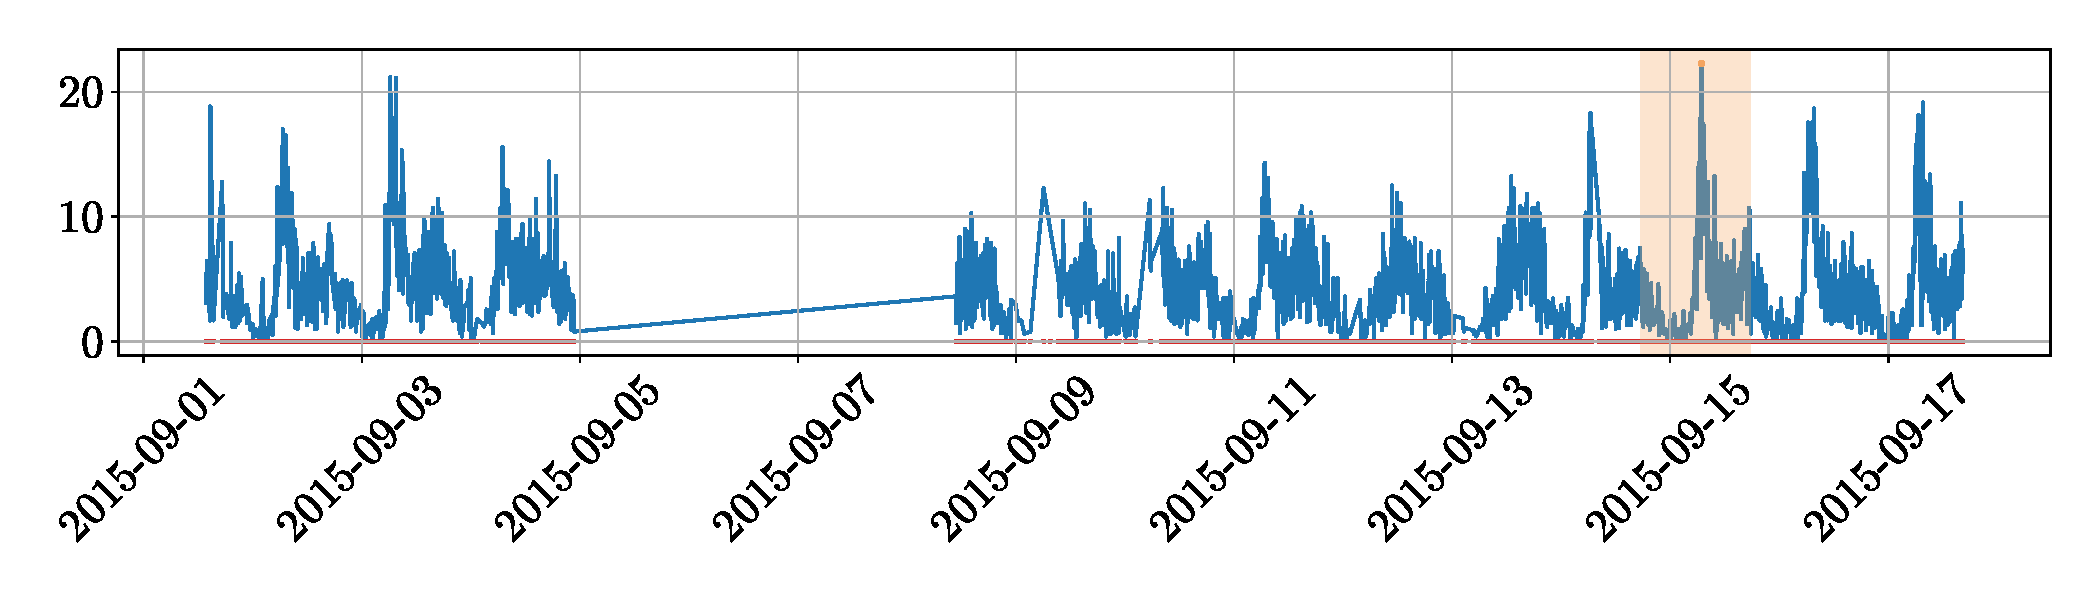
\includegraphics[width=0.8\linewidth]{./img/_md_traffic_data.pdf}
    \caption{
        \parbox[t]{0.7\linewidth}{
            Plot of the data. Straight lines are artifacts of missing values. Red dots below represent the actual data points.
        }
    }
\end{figure}



\section{Preliminaries}

The dataset has sparse indexes (i.e., indexes are non-contiguous) and missing values are represented by gaps. It is necessary to use dense indexes where missing values are explicitly marked as \texttt{NaN}.

\subsection{Resampling / Binning}

\begin{description}
    \item[Resampling / binning] \marginnote{Resampling / binning} 
        Resample the indexes of the dataset so that they have a regular step (e.g., 5 minutes).

        \begin{remark}
            Values that end up in the same bin need to be aggregated (e.g., mean).
        \end{remark}

        \begin{figure}[H]
            \centering
            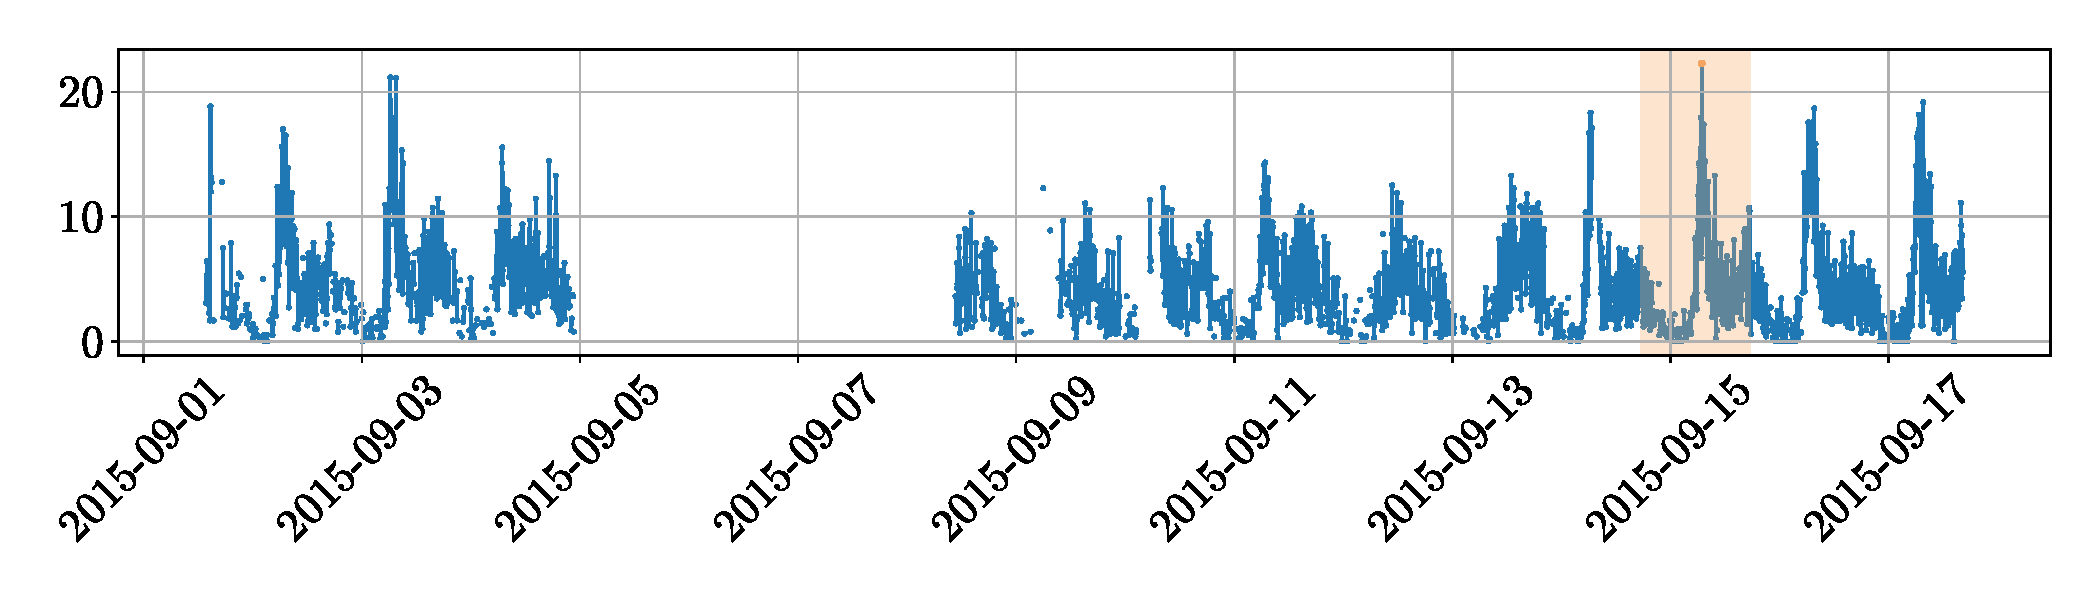
\includegraphics[width=0.8\linewidth]{./img/_md_traffic_resampled.pdf}
            \caption{
                Plot of the resampled data without artifacts
            }
        \end{figure}
\end{description}



\section{Approaches}

\begin{description}
    \item[Benchmark dataset] 
        A portion of known data where some values are artificially removed can be used to evaluate a filling method. As accuracy metric, RMSE can be used.

        \begin{figure}[H]
            \centering
            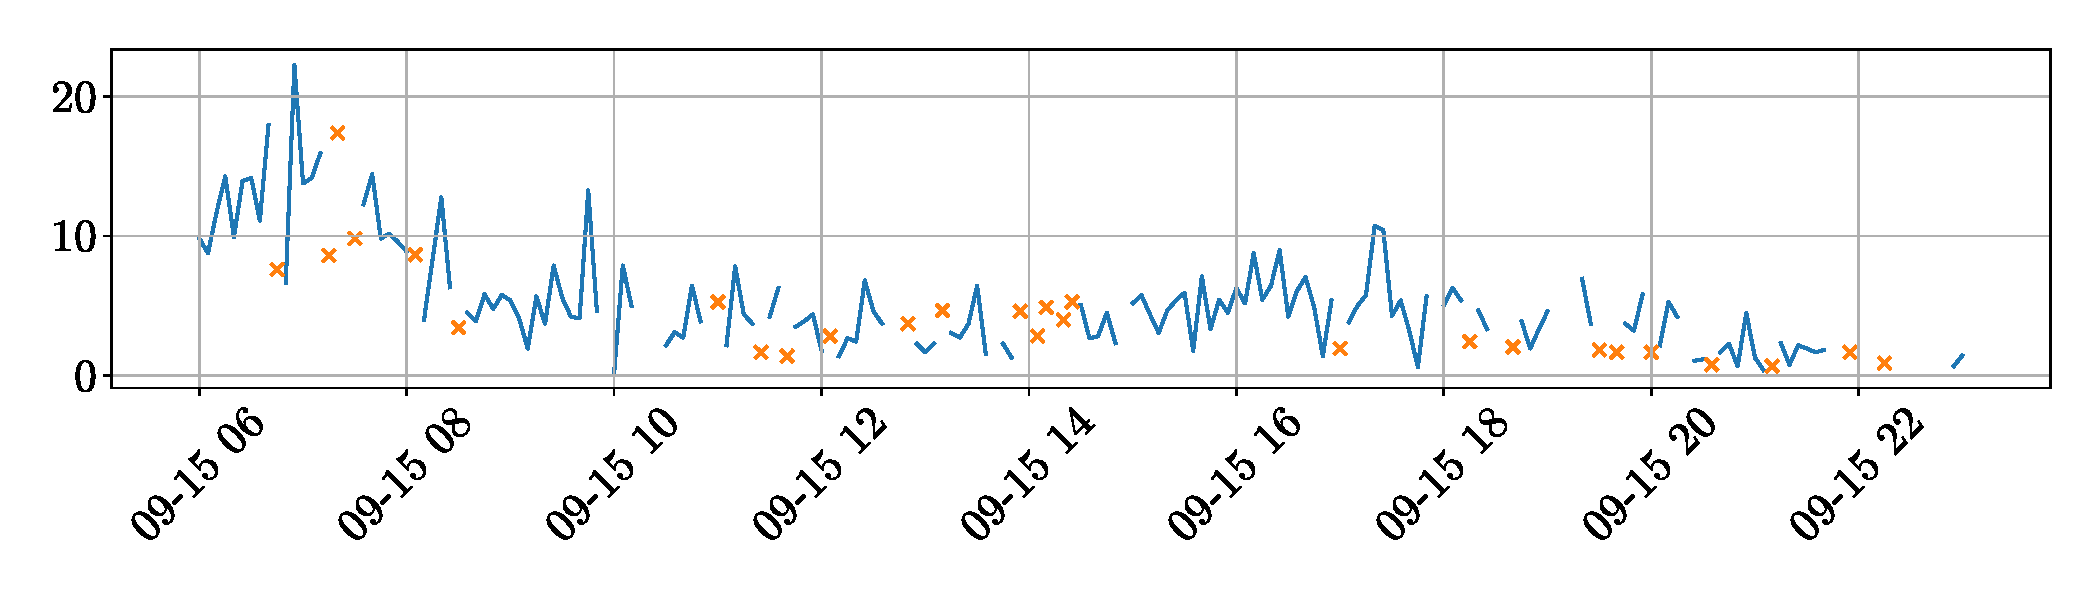
\includegraphics[width=0.8\linewidth]{./img/_md_traffic_eval_data.pdf}
            \caption{Benchmark dataset. Marked points have been artificially removed.}
        \end{figure}
\end{description}


\subsection{Forward/Backward filling}

\begin{description}
    \item[Forward filling] 
        Set the missing value to the last valid observation.

    \item[Backward filling] 
        Set the missing value to the next valid observation.
\end{description}

\begin{remark}
    The idea of this approach is that time series usually have strong local correlation (i.e., some sort of inertia).
\end{remark}

\begin{remark}
    Forward/backward filling tend to work well on low variance portions of the data.
\end{remark}


\subsection{Geometric interpolation}

Interpolate a function to determine missing points. Possible methods are:
\begin{itemize}
    \item Linear,
    \item Nearest value,
    \item Polynomial,
    \item Spline.
\end{itemize}

\begin{remark}
    (R)MSE assumes that the data is normally distributed, independent, and with the same variability at all points. This is not usually true with time series.
\end{remark}


\subsection{Density estimator}

A density estimator can be used to determine a distribution from all the available data. Given an estimator $f(x, \theta)$ for $\prob{x}$, predictions can be obtained through maximum a posteriori (MAP):
\[ \arg\max_{x} f(x, \theta) \]

However, MAP with density estimators is computationally expensive.

\begin{remark}
    Almost all inference approaches in machine learning can be reduced to a maximum a posteriori computation.
\end{remark}


\subsection{Regressor}

A regressor can be used to fill missing values autoregressively through a rolling forecast by repeatedly making a prediction and including the new point as a training sample.

However, regression only relies on the data on one side (past or future) and each autoregressive iteration accumulates compound errors.


\subsection{Gaussian processes}

\begin{remark}
    The ideal estimator is the one that is:
    \begin{itemize}
        \item At least as powerful as interpolation (i.e., considers both past and future data).
        \item Able to detect the expected variability (i.e., a measure of confidence).
    \end{itemize}
\end{remark}

\begin{description}
    \item[Gaussian process] \marginnote{Gaussian process}
        Stochastic process (i.e., collection of indexed random variables) such that:
        \begin{itemize}
            \item The index variables $x$ are continuous and represents an input of arbitrary dimensionality.
            \item The variable $y_x$ represents the output for $x$.
        \end{itemize}

        The random variables $y_x$ respect the following assumptions:
        \begin{itemize}
            \item They follow a Gaussian distribution.
            \item The standard deviation depends on the distance between a point and the given observations (i.e., a confidence measure).
            \item $y_x$s are correlated. Therefore, every finite subset of $y_x$ variables follows a multivariate normal distribution.
        \end{itemize}

        \begin{figure}[H]
            \centering
            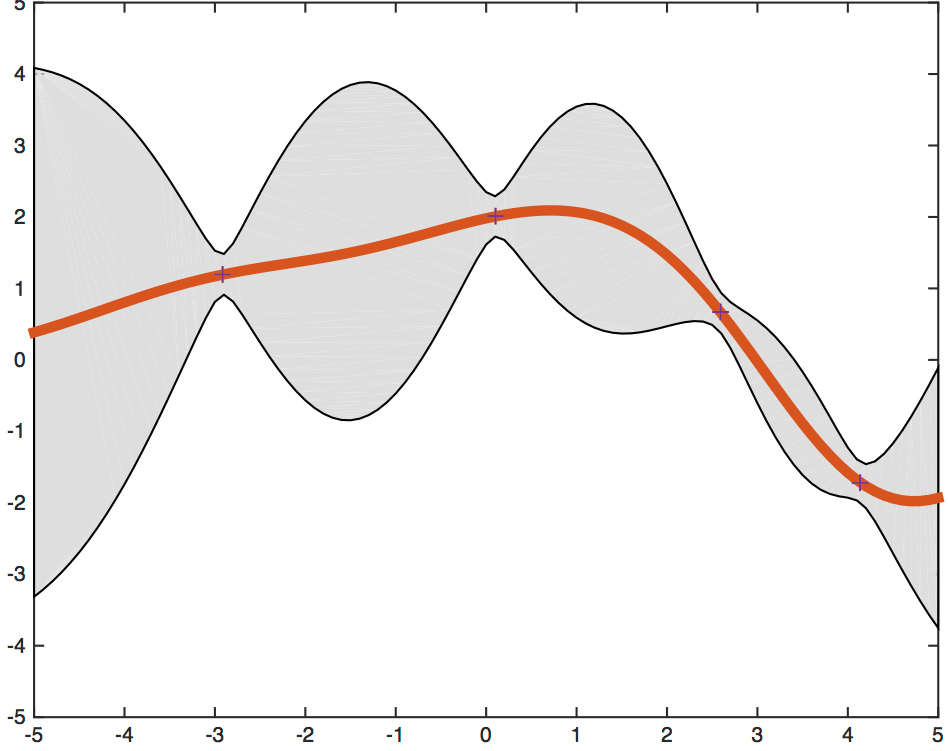
\includegraphics[width=0.4\linewidth]{./img/gp_example.png}
            \caption{
                \parbox[t]{0.6\linewidth}{Example of Gaussian process. The red line represents the mean and the gray area the confidence interval.}
            }
        \end{figure}

        \begin{remark}
            The PDF of a multivariate normal distribution is defined by the mean vector $\vec{\mu}$ and the covariance matrix $\matr{\Sigma}$. By recentering ($\vec{\mu}=\nullvec$), knowing $\matr{\Sigma}$ is enough to compute the joint or conditional density.
        \end{remark}

        \begin{remark}
            To fill missing values, the conditional density $f(y_x | \bar{y}_{\bar{x}})$ is used to infer a new observation $y_x$ given a set of known observations $\bar{y}_x$.
        \end{remark}


    \item[Naive implementation] \phantom{}
        \begin{description}
            \item[Training] 
                Given the training observations $\bar{y}_x$, the covariance matrix can be defined as a parametrized function $\matr{\Sigma}(\theta)$ and optimized for maximum likelihood:
                \[ \arg\max_{\theta} f(\bar{y}_{\bar{x}}, \theta) \]
                where $f$ is the joint PDF of a multivariate normal distribution.

            \item[Inference] 
                To infer the variable $y_x$ associated to an input $x$, the joint distribution $f(y_x | \bar{y}_{\bar{x}})$ has to be computed:
                \[ f(y_x | \bar{y}_{\bar{x}}) = \frac{f(y_x, \bar{y}_{\bar{x}})}{f(\bar{y}_{\bar{x}})} \]
                \begin{itemize}
                    \item $f(\bar{y}_{\bar{x}})$ can be computed using the $\matr{\Sigma}$ determined during training, which is an $n \times n$ matrix assuming $n$ training observations.
                    \item $f(y_x, \bar{y}_{\bar{x}})$ introduces an additional variable and would require an $(n+1) \times (n+1)$ covariance matrix which cannot be determined without further assumptions.
                \end{itemize}
        \end{description}

    \item[Kernel implementation]
        It is assumed that the covariance of two variables can be determined through parametrized kernel functions $K_\theta(x_i, x_j)$.

        \begin{remark}
            Typically, the kernel is a distance measure.
        \end{remark}

        \begin{description}
            \item[Training]
                Given the training observations $\bar{y}_x$ and a parametrized kernel function $K_\theta(x_i, x_j)$, training is done by optimizing the kernel for maximum likelihood (e.g., gradient descent).

                The trained model is represented by both the kernel parameters $\theta$ and the training samples $\bar{y}_x$.

            \item[Inference] 
                Given a new input $x$, the joint distribution $f(y_x | \bar{y}_{\bar{x}})$ can be computed by obtaining $\matr{\Sigma}_{\bar{x}}$ and $\matr{\Sigma}_{x, \bar{x}}$ using the kernel.
        \end{description}

    \item[Common kernels] \phantom{}
        \begin{description}
            \item[Radial basis function] 
                Based on the Euclidean distance $d(x_i, x_j)$ between the input points:
                \[ K(x_i, x_j) = e^{-\frac{d(x_i, x_j)^2}{2l}} \]
                where $l$ is a parameter and represents the scale.

            \item[White kernel]
                Captures the noise in the data:
                \[ K(x_i, x_j) = \begin{cases}
                    \sigma^2 & \text{iff $x_i = x_j$} \\
                    0 & \text{otherwise}
                \end{cases} \]
                where $\sigma$ is a parameter and represents the noise level.

            \item[Constant kernel]
                Represents a learnable constant factor, useful to tune the magnitude of other kernels.

            \item[Exp-Sine-Squared]
                Captures a period:
                \[ K(x_i, x_j) = e^{-2 \frac{\sin^2 \left( \pi \frac{d(x_i, x_j)}{p} \right)}{l^2}} \]
                where $l$ and $p$ are parameters representing periodicity and scale, respectively.

            \item[Dot product]
                Is more or less able to capture a trend:
                \[ K(x_i, x_j) = \sigma^2 + x_i x_j \]
                where $\sigma$ is a parameter and represents the base level of correlation.

                \begin{remark}
                    This kernel is not translation-invariant
                \end{remark}
        \end{description}

        \begin{remark}
            Bounding the domain of the parameters of a kernel can help control training.
        \end{remark}
\end{description}


\begin{remark}
    With Gaussian processes, as we have both the prediction and the confidence interval, likelihood can be used as evaluation metric.
\end{remark}

\begin{remark}
    With Gaussian processes, by predicting points far away from the training observations (i.e., extrapolation), the mean starts to fall to $0$. Only when there is a period, predictions outside the reference observations can be reasonably made.
\end{remark}

\begin{remark}
    As the reference observations and the trained kernel are detached, it is possible to change reference observations without retraining.
\end{remark}

\begin{description}
    \item[Inference]
        As changing reference observations can be done without retraining the kernel, the whole series can be used when doing inference to obtain more accurate results.

        To fill missing values, there are two main strategies:
        \begin{descriptionlist}
            \item[Prediction]
                Use the mean as filling value.

            \item[Sampling]
                Use mean and variance to sample a point to fill the missing value. Clipping might be needed to make the sampled point valid (e.g., prevent negative values for traffic).
        \end{descriptionlist}
        \begin{remark}
            Using the mean results in a smoother filling, while sampling produces more realistic data.
        \end{remark}
\end{description}


\subsection{Multiplicative ensemble}

\begin{remark}
    Gaussian process alone only accounts for covariance and do not consider input-dependent variance (i.e., variance of the traffic at the same week day and time on different days).
\end{remark}

\begin{remark}
    Variance scales via multiplication but not summation:
    \[ Var(x + \alpha) = Var(x) \qquad Var(\alpha x) = \alpha^2 Var(x) \]
    for a constant $\alpha$.
\end{remark}

\begin{description}
    \item[Multiplicative ensemble]
        Product of the outputs of two models $f$ and $g$:
        \[ g(x, \lambda) f(x, \theta) \]
        More specifically, the training process aims to obtain:
        \[ g(x_i, \lambda) f(x_i, \theta) \approx y_i \Rightarrow f(x_i, \theta) \approx \frac{y_i}{g(x_i, \lambda)} \]
        In other words, $f$ is trained on a series with variance altered by $g$.

        For this specific problem, $f$ is a Gaussian process and $g$ a standard deviation model.
\end{description}

\begin{description}
    \item[Standard deviation model] 
        A simple standard deviation model consists of mapping time intervals to their standard deviations. This approach is sensitive to the choice of the granularity of the interval (time unit in this problem):
        \begin{itemize}
            \item If it has too many missing values or too little samples, it is not enough to compute a reliable standard deviation.
            \item If it is too coarse, the computed standard deviation is not useful.
        \end{itemize}

        \begin{remark}
            From empirical considerations, the central limit theorem is observable starting from $30$ samples. Therefore, $30$ data points are enough to make a reasonably stable prediction of the standard deviation.
        \end{remark}

        As the final model might be too coarse, the following can be done:
        \begin{descriptionlist}
            \item[Upsampling] 
                Use a finer grain unit (i.e., x-axis, time unit in this problem) and fill missing values through linear interpolation.

            \item[Smoothing]
                Smooth the upsampled data through a low-pass filter.

                For this problem, an exponentially weighted moving average works best as recent data are more relevant.
        \end{descriptionlist}
\end{description}